\documentclass{article}
\usepackage{amsmath}
\usepackage{graphicx}
\graphicspath{images}
\usepackage{hyperref}
\usepackage{subcaption}


\title{Testing Sorting Algorithms}
\author{Susanne Gjersund}
\makeindex

\begin{document}
	
	
	\maketitle
	\newpage
	\maketitle
	\tableofcontents
	\newpage


\section{Introduction}
	
	Sorting seems to come natural to us humans, it's something we do a lot. We like to arrange things or data in a certain order based on our own criteria. Sometimes to improve the readability of that data, and other times to make it easier and faster to search for or extract specific data.\\
	
	We see it all around us, sorting the bills by value before we count their sum, looking up a word alphabetically in a dictionary, sorting is a processes that can make certain tasks a lot easier and less time consuming.
	
\subsection{Why do we need sorting algorythms}
	
	The same is true for a computer. If we imagine a list of unsorted data, a computer would have to do what we call a linear search. This means it would have to start at the beginning of the list, and look at every single element until it finds the one it's looking for. Of course you might get lucky, but what you're searching for might not even be in that list. In this worst case scenario you would still have to look at every single element.\\
	\\
\textbf{Unsorted: Linear Search}\\
$size = n \rightarrow n  \space comparisons$\\
	
	In terms of processing power and time, when dealing with very big sets of data, this will quickly accumulate, would be far too slow and take up a lot of computational power.
	However, if we were to sort this data before searching, we could for example do a binary search leading to much quicker results.\\
	\\
	\textbf{Sorted: Binary Search}\\
$size = n \rightarrow \log_{2} n \space comparisons$\\

Luckily, a lot of people have spent a lot of time coming up with sorting algorithms that can help us sort our datasets. In fact, there are so many it's easy to lose track and get confused. We'll take a look at a few of the more known and common ones throughout this report, and compare them to see what makes them differ from each other.

	\newpage
\subsection{How I test performance}

I've created a simple QT Application to run and test these algorithms. It might not produce an exact result due to some delays caused by debugging-elements. However, all sorting functions suffer the same delays, so relative to each other they should still be comparable. 

\begin{figure}[h]
	\centering
	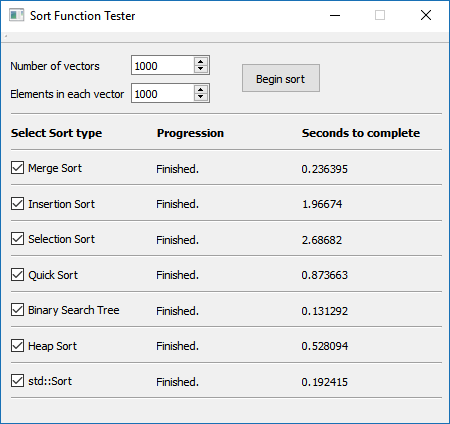
\includegraphics[width=0.7\linewidth]{images/UI}
	\caption[QT Application UI]{QT Application UI}
	\label{fig:ui}
\end{figure}

In figure \ref{fig:ui} you can see the basic layout of the application. In order to handle dynamic arrays sizes, it uses vectors rather than arrays. The user can chose how many vectors to create, and how long each of them will be. This is to be able to better test the difference in performance between the sort functions. One might be better at sorting one very big array, while another may be better at sorting many small arrays. Almost all of the code is written as a template, so it would be easy to make it work on different data types, but for now it fills each vector with an integer between 1 and 100.


	\newpage

\section{The different Sorting Algorithms}

There will be a few collective indications on each sorting function:
\\
\textbf{Time complexity:} Big O notation on the expected runtime 
\\
\textbf{In-Place:} Means that the sorting uses no extra memory


\subsection{Selection Sort}

Selecting sort is one of the simpler sorting algorithms, and is quite intuitive. It uses one array, divided into two subarrays - one sorted subarray that starts off empty and one containing the remaining unsorted subarray. The algorithm repeatedly finds the smallest element in the unsorted subarray and adds it to the sorted subarray by swapping it with the element directly after the highest element in the sorted subarray, until you're eventually left with one fully sorted array.
\\
\textbf{Time Complexity:} $O(n^{2})$ 
\\as there are two nested loops.
\\
\textbf{In Place:} Yes, using only one array it does not require extra space.

\begin{figure}[h]
	\centering
	\includegraphics[width=1\linewidth]{"images/Selection Sort"}
	\caption{Selection Sort Performance}
	\label{fig:selection-sort}
\end{figure}




\subsection{Insertion Sort}

In the same way selection sort consists of two subarrays, so does Insertion sort, one sorted left, and one unsorted right part. At first the sorted subarray contains only one element, and we keep track of where the sorted subarray ends and the unsorted starts. We then take the first element in the unsorted subarray, and going left compare it to the elements in the sorted subarray one by one. The goal is to insert the element at the correct position, and to do this it swaps places with the element on its left until it finds an element smaller than itself. Then we look at the next unsorted card, repeating this process leaves us with a fully sorted array.

Insertion sort can be used when number of elements is small. It can also be useful when input array is almost sorted, only few elements are misplaced in complete big array. Insertion sort takes maximum time to sort if elements are sorted in reverse order. And it takes minimum time (Order of n) when elements are already sorted.
\\
\textbf{Time Complexity:} $O(n^{2})$\\
It is still better than Selection Sort because it requires fewer swaps on average
\\
\textbf{In-Place:} Yes, only uses one array

\begin{figure}[h]
	\centering
	\includegraphics[width=1\linewidth]{"images/Insertion Sort"}
	\caption{Insertion Sort Performance}
	\label{fig:insertion-sort}
\end{figure}




\subsection{Merge Sort}

Unlike the two previous algorithms, Merge sort is a recursive algorithm, reducing itself in a self-similar manner. It operates by spitting the original unsorted array into two equal arrays and then repeats by further splitting those two into four new ones, this goes on until we're left with arrays of only single elements. We then merge two and two arrays by comparing their leftmost untouched index's data, whichever is smallest overwrites the leftmost unsorted index of the array they once split from. By doing this, we reduce the problem to sub problems, sorting the children and merging them to replace the parent. This all happens recursively, so we focus on one split array at a time, and when the parent is sorted, and we're done with the child, we delete it from memory before moving on.
\\
\textbf{Time complexity:} $O(n\log n)$\\
in all 3 cases (worst, average and best) as merge sort always divides the array in two halves and take linear time to merge two halves.
\\
\textbf{In-Place:} No, Creates new arrays when sorting, so uses more memory.

\begin{figure}[h]
	\centering
	\includegraphics[width=1\linewidth]{"images/Merge Sort"}
	\caption{Merge Sort Performance}
	\label{fig:merge-sort}
\end{figure}


\newpage

\subsection{std::Sort}

std::sort() is C++ Standard Library's generic sort function. It uses something called Intro Sort, which is a hybrid algorithm, meaning that it uses more than one sorting algorithm. By using three sorting algorithm to minimise the running time, Quicksort, Heapsort and Insertion Sort, it's possibly the best algorithm there is.
\\
\textbf{Time complexity:} $O(n\log n)$
\\
\textbf{In Place:} Yes


\begin{figure}[h]
	\centering
	\includegraphics[width=1\linewidth]{"images/std Sort"}
	\caption{std::Sort Performance}
	\label{fig:std-sort}
\end{figure}




\subsection{Binary Search Tree}

A binary search tree does not use an array like the other sorting functions mentioned here, instead it sets up a node-based binary tree data structure with the following properties:
\\The left subtree of a node contains only nodes with keys lesser than the node’s key.
\\The right subtree of a node contains only nodes with keys greater than the node’s key.
\\The left and right subtree each must also be a binary search tree.
\\So when sorting using this method we don't actually restructure an array, though we can collect data from an array and insert it into the binary tree. The sorting has to do with how we collect data from the tree once it's filled, by traversing in a certain order we can easily collect the data and place it back into the original array fully sorted.
Depending on what you want, an array would usually be preferable since it's elements are placed in consecutive order in memory, while nodes in a binary tree can be random. However binary trees does have the advantage that they are always sorted.
\\
\textbf{Time complexity (insert) Average:} $O(\log n)$\\

\begin{figure}[h]
	\centering
	\includegraphics[width=1\linewidth]{"images/Binary Search Tree"}
	\caption{Binary Search Tree Performance}
	\label{fig:binary-search-tree}
\end{figure}

\subsection{Heap Sort}

Just like a Binary Search Tree, Heap sort doesn't use an array but instead it's own binary tree data structure using either one of these properties:
\\Max heap: A parent node needs to be larger than it's children
\\Min heap: A parent node needs to be smaller than it's children
\\However, because of it's structure and the way it always fills the next empty node to create a Complete Binary Tree, it is often represented as an array. This is because we can calculate what position in an array correspond to which node on a filled binary tree. If the parent node is at index i, and indexing starts at 0:
\\$left child = 2 \times i + 1$
\\$right child = 2 \times i + 2$
\\It is similar to selection sort in that it uses a sorted and unsorted part, finds the largest element and places it at the end of the heap. This process is repeated until the heap is fully sorted.
\\
\textbf{Time Complexity:} $O(n\log n)$.
\\\textbf{In-Place:} Yes

\begin{figure}[h]
	\centering
	\includegraphics[width=1\linewidth]{"images/Heap Sort"}
	\caption{Heap Sort Performance}
	\label{fig:heap-sort}
\end{figure}

\newpage
\section{Conclusion}

Looking at these different performances side by side like in figure \ref{fig:dataset} it's easy to see that std::Sort by far outperforms the rest when it comes to large sets of data. However, when sorting smaller sets of data as seen in figure \ref{fig:dataset} it doesn't really matter, they all perform quite well. Using the std::sort as a standard could be a good idea, as it performs the best in all shown cases, also when dealing with multiple datasets as seen fin \ref{fig:several-vectors}.
\begin{figure}[h]
	\begin{subfigure}{\linewidth}
		\includegraphics[width=0.5\linewidth]{"images/small dataset"}\hfill
		\includegraphics[width=0.5\linewidth]{"images/large dataset"}\hfill
	\end{subfigure}\par\medskip
	\label{fig:dataset}
	\caption{Left: Small dataset, Right: Large dataset}
\end{figure}

\begin{figure}
	\centering
	\includegraphics[width=0.7\linewidth]{"images/several vectors"}
	\caption{More than one dataset}
	\label{fig:several-vectors}
\end{figure}




\end{document}